\documentclass{mcmthesis}
\usepackage{float}
\mcmsetup{
  tcn=2224715,
  problem=A,
  sheet=true,
  titleinsheet=true,
  keywordsinsheet=true,
  titlepage=true,
  abstract=true
}

\makeatletter
\newcommand{\thickhline}{%
    \noalign {\ifnum 0=`}\fi \hrule height 1pt
    \futurelet \reserved@a \@xhline
}
\makeatother

\title{Replace with your title}

\begin{document}
  \begin{abstract}
    This is the abstract.
  \end{abstract}

  \begin{keywords}
    keyword1, keyword2
  \end{keywords}
  \maketitle
  \tableofcontents
  \clearpage
  \section{Introduction}
  \subsection{Problem Background}
  Since the first bicycle race was held on the 31 May 1868 at the Parc de Saint-Cloud, Paris, various bicycle games have emerged in large numbers, including road bicycle, tracking cycling, mountain bike and so on. In different kinds of bicycle race, riders are always looking to minimize the time required to cover a given distance.\\
  Besides the fitness of the athletes, appropriate strategies also play a decisive role in a cycling race. A rider can keep a constant speed in the whole game. And he can adjust his speed according to the landform and wind, as well. He can exceed his limits under a certain condition at the price of riding slowly in the next period.\\ 
  However, everyone has different properties in riding. For example, someone may specialize in races that have multiple long climbs (a climber), while another specializes in producing extremely high power for short periods of time (a sprinter). This difference can be described as discrepancy in power curve, which indicates how long a rider can produce a given amount of power. Given a particular rider’s capability according to that rider’s power curve, how should that rider apply power while traversing a given time trial course? \\
  kMoreover, in a team time trial, a team often ride in a line to reduce the air resistance. Given that the team consists of different type of riders, how to arrange the speed of the team and how to arrange the lead rider? These questions are discussed in this paper.\\
  \subsection{Problem Restatement}
  \begin{enumerate}
    \item Develop a model that can be applied to any type of rider that determines the relationship between the rider’s position on the course and the power the rider applies.
    \item Define the power profiles of riders of different types and different genders.
    \item Apply the model on various time trial courses.
    \item Determine the potential impact of weather conditions.
    \item Determine how sensitive the results are to rider deviations from the target power distribution.
    \item Discuss how to extend your model to include the optimal power use for a team time trial.
    \item Write a two-page rider’s race guidance for a Directeur Sportif of a team.
  \end{enumerate}
  
  \subsection{Our Approach}

  \section{Data}
  \subsection{Data Collection}
  The data we used mainly include geographic information of the racing course, typical power curves of different kinds of cyclists.
  The data sources are summarized in Table \ref{tab:data_source}.
  \begin{table}[H]
    \centering
    \caption{Data source collation}
    \label{tab:data_source}
    \begin{tabular}{ccc}
    \thickhline
    Database Names & Database URL & Data Type \\\hline
    Google Earth & \href{https://earth.google.com}{https://earth.google.com} & Geography \\
    SRTM1 & \href{https://www2.jpl.nasa.gov/srtm}{https://www2.jpl.nasa.gov/srtm} & Geography \\
    ODP1 & \href{https://data.opendataportal.at/dataset/dtm-europe}{https://data.opendataportal.at/dataset/dtm-europe} & Geography \\
    \thickhline
    \end{tabular}
  \end{table}

  \subsection{Data Process}

  \subsubsection{Geographic information of the racing course}
  To get the 3D model of the cycling course, we looked up the rider manual. We uniformly sampled points on the racetrack and marked them on Google Earth. In this way, the longitude and latitude information can be exported. Then we reached the elevation information of these points using the database SRTM1 and ODP1.\\
  In order to simplify the data process procedure, we transform the course from terrestrial coordinate system to a space rectangular coordinate system, whose origin locates at the start point and whose $x'$, $y'$, $z'$ axis orient to south, east, sky respectively. The detailed procedures are shown in Fig. \ref{fig:img1}
  \begin{figure}[H]
    \centering
    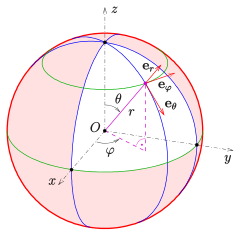
\includegraphics[width=0.4\linewidth]{image/earth_coord}
    \caption{Schematic diagram of the relationship between the ground coordinate system and the right angle coordinate system}%
    \label{fig:img1}
  \end{figure}

  In the old coordinate system shown as $C_{xyz}$ , the coordinate of the start point can be represented as:
  \begin{equation}
    \begin{aligned}
      r_{0} = r_0 \sin \theta_0 \cos \varphi_{0} \hat{x} + r_0 \sin \theta_0 \cos \varphi_0 \hat{y} + r_0 \cos \theta_{0} \hat{z}
    \end{aligned}
  \end{equation}
  where $r_0$ is the coordinate vector of start point in the $C_{xyz}$, $r_0$ is the distance between the start point and he center of the earth $r_0 = R_{e} + h_0$, $R_{e}$ is the radius of the earth, $h_0$ is the elevation of start point; $\theta_0 = \text{latitude-of-startpoint} - 90^\circ$; $\varphi_0$ is he longitude of start point.\\
  The new coordinate is shown in the figure, $C_{e_\theta e_\varphi e_r}$, Its basis vectors can be represented as:
  \begin{equation}
    \left\{
    \begin{aligned}
      &{\bf \hat{e}_{\theta}} = \frac{\sin \theta_0}{|\sin \theta_0|} \cos \theta_0\cos \varphi_0 {\bf \hat{x}} + \frac{\sin \theta_0}{|\sin \theta_0|}\cos \theta_0 \sin\varphi_0 {\bf \hat{y}} - \frac{\sin \theta_0}{|\sin \theta_0|}\sin \theta_0 {\bf \hat{z}} \\
      & {\bf \hat{e}_{\varphi}} = -\sin \varphi_0 {\bf \hat{x}} + \cos \varphi_0 {\bf \hat{y}}\\
      & {\bf \hat{e}_{r}} = \sin \theta_0 \cos \varphi_0 {\bf \hat{x}} + \sin \theta_0 \cos \varphi_0 {\bf \hat{y}} + \cos \theta_{0} {\bf \hat{z}}
    \end{aligned}
    \right.
  \end{equation}
  For the points in he course,
  \begin{equation}
    \begin{aligned}
      {\bf r} &= r\sin \theta \cos \varphi {\bf \hat{x}} + r\sin \theta \cos \varphi {\bf \hat{y}} + r\cos \theta {\bf \hat{z}}\\
              &= ({\bf r}\cdot {\bf \hat{e}_{\theta}}) {\bf \hat{e}_{\theta}} + ({\bf r}\cdot {\bf \hat{e}_{\varphi}}){\bf \hat{e}_{\varphi}} + ({\bf r}\cdot {\bf \hat{e}_{r}}){\bf \hat{e}_{r}}\\
              &= ({\bf r}\cdot {\bf \hat{e}_{\theta}}) {\bf \hat{x}'} + ({\bf r}\cdot {\bf \hat{e}_{\varphi}}) {\bf \hat{y}'} + ({\bf r}\cdot {\bf \hat{e}_{r}}){\bf \hat{z}'}
    \end{aligned}
  \end{equation}

  The coordinate of the points in the new coordinate system is $({\bf r}\cdot {\bf \hat{e}_{\theta}}, {\bf r}\cdot {\bf \hat{e}_{\varphi}}, {\bf r}\cdot {\bf \hat{e}_{r}})$.\\

  As we can see, there are plenty of spines on the figure. The fluctuation of the coordinate is caused of the point sampling on the map. The unrealistic ascent and descent will disturb our simulation to a large extent. To avoid this this problem, we smoothed the data using Gaussian convolution. \\
  For a set of 2-dimensional data $(\xi_{i}, \zeta_{i})$, we can smooth the data with method of weighted average. The weight can be the Gaussian distance between indicator. In this way, the smoothed data can be presented as $(\xi_{j}, \zeta_{j})$ in which
  \begin{equation}
    \begin{aligned}
      \zeta_{j} = \frac{\sum_{i} \zeta_{i} e^{-\frac{(\xi_{i} - \xi_{j})^2}{2 \sigma^{2}}}}{\sum _{i} e^{- \frac{(\xi_{i} - \xi_{j})^{2}}{2 \sigma^{2}}}}
    \end{aligned}
  \end{equation}


  \end{document}
